\section{Geography-Aware Self-Supervised Learning}
\label{sec:methodology}

This section provides a brief introduction to the geography-aware contrastive learning approach presented in \cite{geoAwareSelfSuper}. Initially, they evaluated the state-of-the-art self-supervised contrastive learning method, MoCo-v2 \cite{mocoV2}, on remote sensing datasets such as the Functional Map of the World (fMoW) image classification benchmark \cite{fmow}. The evaluation revealed a performance gap between the self-supervised learning and supervised learning using labels. \\
To bridge this gab they introduced geography-aware contrastive learning to leverage the spatio-temporal structure of remote sensing data. Unlike contrastive learning for traditional computer vision images where different views of the same image serve as a positive pair as in MoCo-v2, they propose to use temporal positive pairs from spatially aligned images over time. By doing so, the representations tent to be invariant to subtle variations over time, e.g. to seasons or weather. \\
They further designed an unsupervised learning method that uses geo-location information as a pre-text task. The task is to predict where in the world an image comes from. Models performing well in that task should be able to identify visual cues that are transferable to other downstream tasks. Both methods can be integrated into a single geography-aware contrastive learning objective. \\


\begin{figure}[t]
  \centering
   %\fbox{\rule{0pt}{1.5in} \rule{0.9\linewidth}{0pt}}
   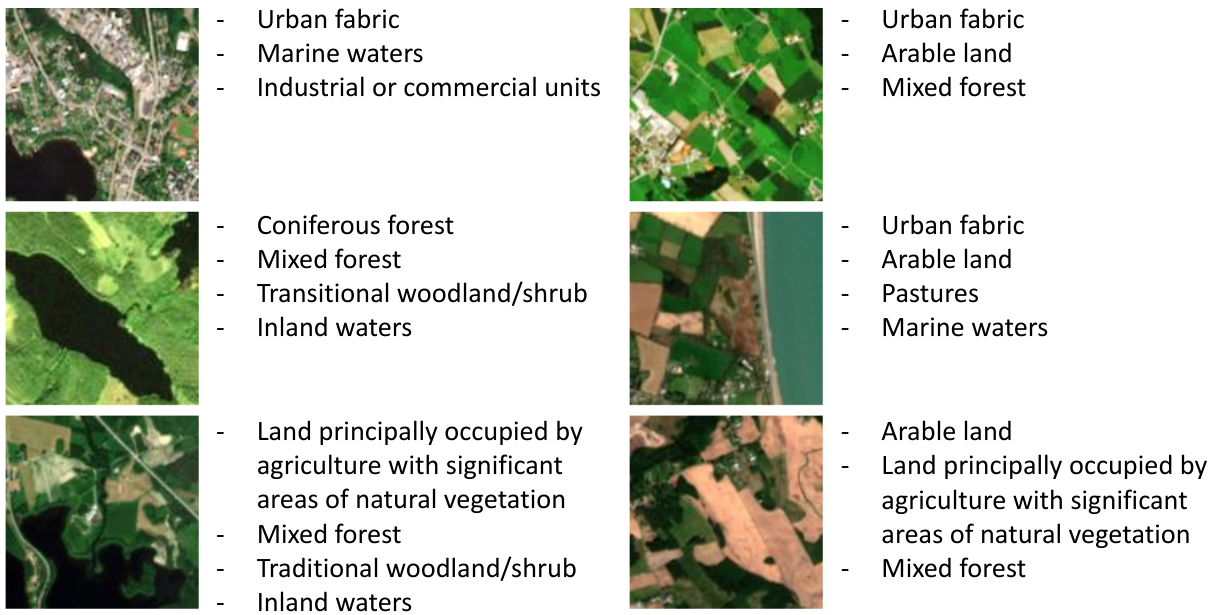
\includegraphics[width=\linewidth]{figures/BigEarthNet.png}
   \caption{Examples of Sentinel-2 images and their multi-lables in the BigEarthNet-MM dataset (adapted from \cite{BigEarthNetImg}).}
   \label{fig:BigEarth}
\end{figure}

\subsection{Contrastive Learning with temporal positive pairs}

The authors consider a geo-tagged visual dataset $\{((x_i^1, ..., x_i^{T_i}), $lat$_i, $lon$_i)\}_{i=1}^N$ where the $i$th datapoint consists of a sequence of images $(x_i^1, ..., x_i^{T_i})$ at a shared loaction with latitude (lat) and longituda (lon) over time $t_i = 1, ..., T_i$. The fMoW dataset fits these criteria. \\
Contrastive methods define a mapping $f_q: x_i^t \mapsto z_i^t \in \mathbb{R}^d$ from pixels $x_i^t$ to latent representations $z_i^t$. Models should learn representations by pulling positive images pairs from the same instance closer in latent space while pushing negative pairs from different instantes further away. \\
The Moco-v2 and the geography-aware contrastive learning framework are shown in Fig. \ref{fig:Moco} and Fig. \ref{fig:geography_aware}.
The objective is defined as follows \cite{geoAwareSelfSuper}:
\begin{equation}
    \label{eq:contrastive_loss}
    L_z = - \log\frac{\exp(z\cdot z'/\lambda)}{\exp(z\cdot z'/\lambda) + \sum_{j=1}^N \exp(z\cdot k_j/\lambda)},
\end{equation}
where $z$ and $z'$ are the encoded representations of a positive data pair $v$ and $v'$. $N$ is the number of negative samples, $\{k_j\}_{j=1}^N$ are the encoded negative pairs and $\lambda\in\mathbb{R}^+$ is the temperature hyperparameter. The similarity of the representations is measured by the dot product. \\
In MoCo-v2 the positive pair $v$ and $v'$ are two augmented views of an image $x_i^t$. Ayush et al. \cite{geoAwareSelfSuper} create positive pairs from a sequence of images $(x_i^1, ..., x_i^{T_i})$ by selecting a random image $x_i^{t_2}$ to pair with a given image $x_i^{t_1}$. They then apply pertubations like random color jittering to the spatially aligned image pair $x_i^{t_1}$ and $x_i^{t_2}$ resulting in the \textit{temporal positive pair} $v$ and $v'$. For training $v$ and $v'$ are passed through query and key encoders, $f_q$ and $f_k$, respectively.

\subsection{Combining Geo-location Classification and Contrastive Learning}

The geo-location classification pre-text task aims to further improve the quality of the representations. Ayush et al. \cite{geoAwareSelfSuper} cluster the images in the dataset using the coordinates $($lat$_i,$ lon$_i)$. They construct $K$ clusters with a clustering method and assign the areas a categorical geo-label $c_i\in\{1, ..., K\}$. By doing so, they are able to train a geo-location predictor CNN using cross entropy loss. \\
To combine both approaches they use the latent features $z_i^t$ from the contrastive learning query encoder as the input to the geo-location prediction network as shown in Fig. \ref{fig:geography_aware}. They perform joint learning by defining the final loss as the linear combination of the contrastive learning loss $L_z$ in Eq. \ref{eq:contrastive_loss} and the negative cross-entropy loss $L_g$ of the geo-location network with coefficients $\alpha$ and $\beta$: $L_f = \alpha L_z + \beta L_g$. \\
By minimizing $L_f$ they learn representations to jointly maximize agreement between spatio-temporal positive pairs, minimize agreement between negative pairs and predict the geo-label of the images from the positive pairs.

\begin{figure*}[t]
  \centering
   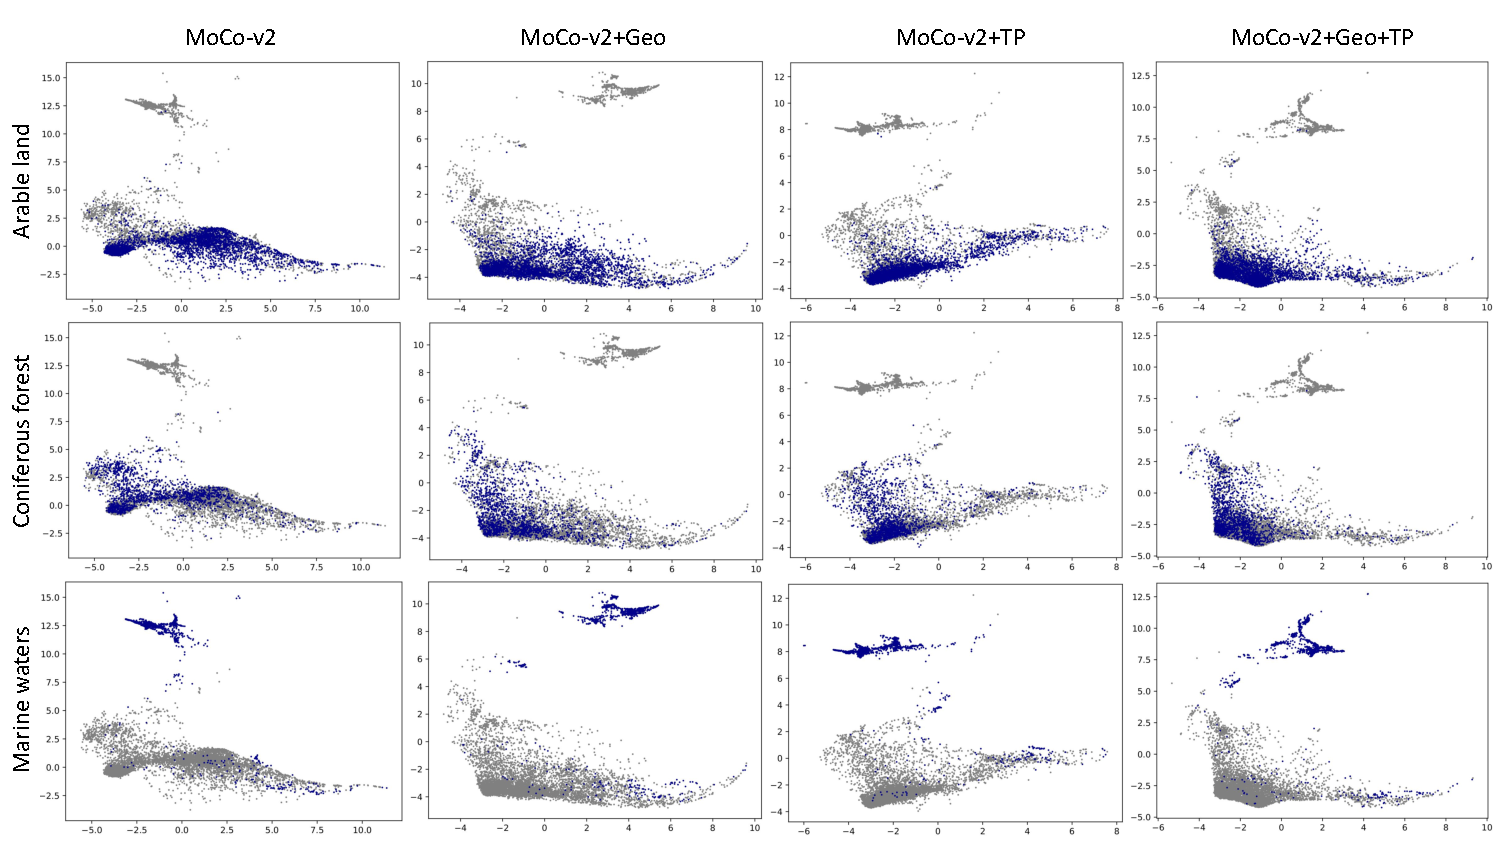
\includegraphics[width=\linewidth]{figures/UMAPVisualization.pdf}
   \caption{UMAP feature visualization of the BigEarthNet test data's feature vectors of the four foundation models. Data points corresponding to the labels \textit{arable land}, \textit{coniferous forest}, and \textit{marine waters} are highlighted in blue.}
   \label{fig:umap}
\end{figure*}